\chapter{Componentes Pasivos}

\section{Resistencias}

La resistencia es la propiedad física de un material que se opone al paso de la corriente. Es el grado de dificultad que los electrones de la banda de conducción encuentran para desplazarse. Supone una pérdida de energía en forma de calor (Efecto Joule). Su valor depende de:

\begin{itemize}
    \item Tipo de material: resistividad \(\rho\)
    \item Temperatura de funcionamiento
    \item Dimensiones físicas del componente
\end{itemize}

\subsection{Definición}
Constante que depende del tipo de material, de sus características eléctricas (resistividad) y de su geometría (longitud y sección).

\begin{equation}
    R = \rho \frac{L}{S}
\end{equation}

Donde:
\begin{itemize}
    \item \(\rho\): resistividad del material conductor
    \item L: longitud del conductor
    \item: S: sección del conductor
\end{itemize}

El valor óhmico de una resistencia relaciona la intensidad que circula a través de ella ($A$), y la tensión desarrollada en sus bornas ($V$).

La constante de proporcionalidad $R$ es la resistencia eléctrica del elemenro y su unidad de medida en el S.I. es el Ohmio y su símbolo es $\Omega$

\begin{equation}
    R[\Omega] = \frac{V[V]}{I[A]}
\end{equation}

\subsection{Parámetros Característicos}

\begin{itemize}
    \item Valor nominal (Rn): Valor teórico nominal de la resistencia (se mide en ohmios). Están tabulados en valores normalizados.
    \item Tolerancia (T\%): Desviaciones superior e inferior sobre el valor nominal. $\pm 20\%,\pm 10\%,\pm 5\%,\pm 1\%,\pm 0.5\%,\pm 0.1\% $
    \item Coeficiente de tensión (Cv): Relación entre la variación relativa de la resistencia y la variación de la tensión que la ha provocado:
    \begin{equation}
        Cv = \frac{\frac{\Delta R}{R}}{\Delta V} (10^6)
    \end{equation}
    \item Potencia nominal (Pn): Potencia en Watios que el elemento puede disipar de una manera continua sin sufrir deterioro, a la temperatura nominal de servicio. Valores normalizados son: $1/8, 1/4, 1/2, 1, 2, 4, 8, 16\ Watios$
    \item Temperatura nominal de funcionamiento: Temperatura ambiente a la cual se define la disipación nominal.
    \item Temperatura máxima de funcionamiento: Temperatura ambiente máxima a la cual puede ser utilizada la resistencia. Cuando la temperatura aumenta, hay que disminuir la potencia nominal admisible, con el objeto de mantener la temperatura de la resistencia dentro de los límites admisibles..
    \item Coeficiente de temperatura ($\alpha$): Variación de la resistencia con la temperatura. Se mide en $\% / ^\circ C$ ó en $ppm / ^\circ C$.
    \begin{equation}
        R_t = R_0 (1 + \alpha t)
    \end{equation}
    \item Resistencia de aislamiento: Valor de la resistencia a la cual son aplicables los ensayos de resistencia de aislamiento y rigidez dieléctrica
\end{itemize}

\subsection{Resistencias fijas through-hole}
\subsubsection{Proceso de fabricación}
\begin{figure}[H]
    \centering
    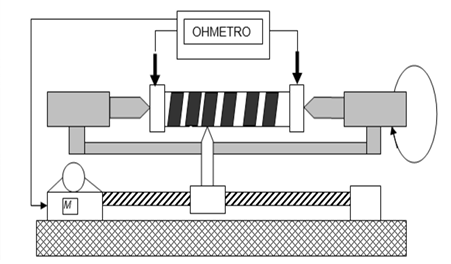
\includegraphics[width=0.5\linewidth]{Imagenes/Resistencias Through Hole - Proceso de Fabricacion.png}
    \caption{Resistencias fijas through-hole. Proceso de Fabricación.}
\end{figure}

\begin{enumerate}
    \item Preparación del núcleo cerámico.
    \item Depósito de carbón por pirólisis.
    \item Fijación de casquillos terminales.
    \item Espiralado.
    \item Soldadura de hilos terminales (patillas).
    \item Recubrimiento aislamiento y pintado del código de colores.
\end{enumerate}

\subsection{Resistencias fijas SMT}
Encapsulado específico para montaje superficial.

\begin{figure}[H]
    \centering
    \begin{subfigure}[c]{0.45 \textwidth}
        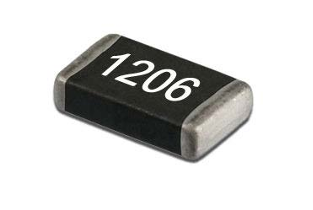
\includegraphics[width=\textwidth]{Imagenes/Resistencias SMT - Encapsulado.png}
        \caption{Encapsulado.}
    \end{subfigure}
    \hfill
    \begin{subfigure}[c]{0.45 \textwidth}
        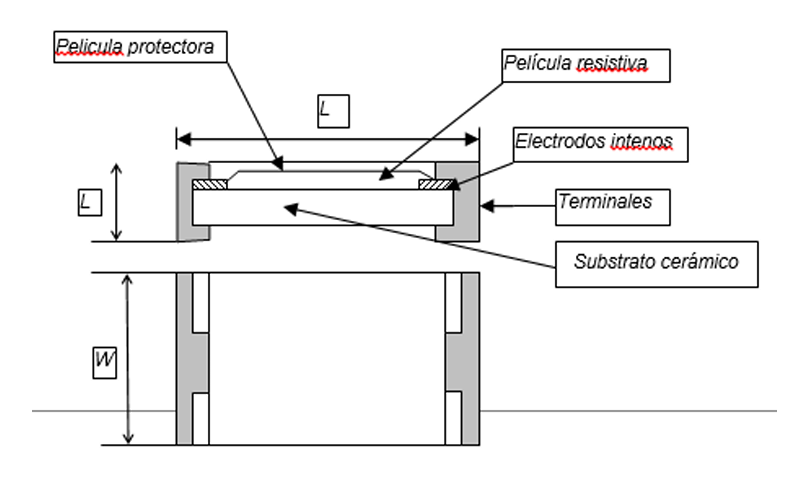
\includegraphics[width=\textwidth]{Imagenes/Resistencias SMT - Estructura Interna.png}
        \caption{Estructura Interna.}
    \end{subfigure}
    \caption{Resistencia SMT.}
\end{figure}

\subsubsection{Proceso de fabricación}

\begin{figure}[H]
    \centering
    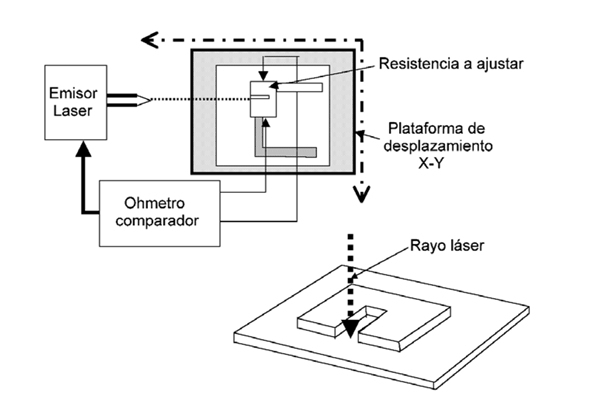
\includegraphics[width=0.5\linewidth]{Imagenes/Resistencias SMT - Proceso de Fabricacion.png}
    \caption{Resistencias fijas SMT. Proceso de Fabricación.}
\end{figure}

\begin{enumerate}
    \item El óhmetro mide valor real y lo compara con el valor teórico.
    \item El proyectos láser emite un haz que elimina el material resistivo.
    \item El resistor sufre el ataque del láser hasta alcanzar el valor deseado.
\end{enumerate}

\subsection{Resistencias variables no lineales}

Componentes resistivos cuya resistencia varia de forma no lineal cuando están sometidos a un parámetro físico.

\begin{itemize}
    \item Termistores: Su resistencia varía con la temperatura. 
    \begin{itemize}
        \item PTC (coeficiente positivo).
        \item NTC (coeficiente negativo).
    \end{itemize}
    \item LDR: Varían con la intensidad lumínica.
    \item VDR: Varían con la tensión aplicada.
\end{itemize}

\subsubsection{Termistores PTC}

El termistor PTC es un dispositivo semiconductor cuya resistencia varía con la temperatura. Posee un coeficiente de temperatura positivo elevado en un intervalo generalmente estrecho de temperaturas. Se fabrican con material cerámico impregnado de Titanato de Bario, impurificado con Titanatos de plomo o circonio. Esto hace que la cerámica (muy aislante) se haga conductora.

Pueden funcionar en carga ó sin carga (modo potencia cero). Al trabajar en carga, hay que tener en cuenta el efecto de autocalentamiento, que va a afectar a su valor resistivo.

El coeficiente de temperatura $\alpha$ es el cambio relativo de su resistencia en relación al cambio de temperatura:

\begin{equation}
    \alpha = \frac{ln(\frac{R_2}{R_1})}{T_2 - T_1}
\end{equation}

\begin{equation}
    R_2 = R_1 \cdot e ^ {\alpha (T_2 - T_1)}
\end{equation}

\subsubsection{Termistores NTC}

Son dispositivos semiconductores, con coeficiente de temperatura negativo (NTC = Negative Temperature Coefficient). Su resistencia decrece conforme aumenta la temperatura. Están elaborados a partir de una mezcla de semiconductores policristalinos, tales como Cromo (Cr), Manganeso (Mn), Hierro (Fe), Cobalto (Co) y Níquel (Ni).

\textbf{Ecuaciones características:}

\begin{equation}
    R_T = Ae^{\frac{B}{T}}
\end{equation}

\begin{equation}
    R_T = R_{25} e ^ {B (\frac{1}{T} - \frac{1}{298,15})}
\end{equation}

\begin{equation}
    \alpha_R = \frac{1}{R_T} \frac{\Delta R_T}{\Delta T}
\end{equation}

Donde:
\begin{itemize}
    \item $R_T$: Resistencia a la temperatura $T$ ($^\circ K$)
    \item $R_{25}$: Resistencia  al temperatura de $25^\circ C$ ($289,15 ^\circ K$)
    \item $A$: Constante del material ($\Omega$)
    \item $B$: Constante específica del material ($K$)
    \item $T$: Temperatura de trabajo ($^\circ K$)
    \item $\alpha_R$: Coeficiente de temperatura del termistor
\end{itemize}

\subsubsection{LDR}

Las fotoresistencias (LDR - Light Dependent Resistor) se basan en la variación de la resistencia eléctrica de un semiconductor al incidir en él la radiación óptica. En un semiconductor, la mayoría de los portadores se hallan, en reposo, en la banda de valencia, existiendo poca densidad de electrones en la banda de conducción. Cuando son sometidos a radiación, los electrones migran a la banda de conducción. La energía para que estos portadores pasen a la banda de conducción puede venir de diversas fuentes, entre las que están la radiación óptica.

\textbf{Fabricación:}
\begin{itemize}
    \item Se utilizan materiales con propiedades fotoconductoras de materiales como el sulfuro de cadmio (SCd), seleniuro de cadmio (SeCd) o el sulfuro de plomo (SPb).
    \item La mezcla de polvo y conglomerante se prensa en forma de tabletas, que se sinterizan.
    \item Se depositan sobre la superficie los electrodos en forma de peine.
    \item El conjunto se cubre con resina transparente o cápsula de vidrio o plástico.
\end{itemize}

\textbf{Ecuación característica:}

\begin{equation}
    R = A \cdot L ^{-\alpha}
\end{equation}

Donde:
\begin{itemize}
    \item $R$: Resistencia en ohmios de la LDR
    \item $A$: Constante que depende de las propiedades internas del material
    \item $L$: Iluminación incidente en Flux (candela)
    \item $\alpha$: Parámetro que depende del material (entre 0,7 y 0,9)
\end{itemize}

\textbf{Unidades:}
\begin{itemize}
    \item Candela (cd): Unidad de intensidad lumínica en una dirección dada. Intensidad de radiación en una dirección perpendicular a una superficie de $1/6000000\ m^2$, de un cuerpo negro a la temperatura de solidificación del Pt ($1770 ^\circ C$) y a una presión de $101,325\ N/m^2$.
    \item Footcandle (fc ó ftc): Unidad de intensidad lumínica medida en $lumenes/pie^2$. Brillo de una vela a una distancia de un pié (0,3 m) $ftc = 10,7639 lux$.
    \item Lumen (lm): Unidad de flujo luminoso.
    \item Lux (lx): Unidad de iluminación igual a un lumen por m2. Equivalente métrico de ftc (Un lux equivale a 0,0929 ftc).
\end{itemize}

\subsubsection{VDR}

Los varistores (VDR - Voltage Dependent Resistors) son dispositivos de protección contra sobretensión. Su valor óhmico disminuye con la tensión. Trabajan en un amplio rango de tensiones, absorben gran cantidad de energía, y apenas consumen cuando no actúan. Se fabrican con Óxido de Zinc molido y mezclado, al que se añade un aglutinante cerámico para conseguir la máxima homogeneidad. Esta mezcla se prensa en forma de discos, que se cuecen a temperatura controlada.

\textbf{Proceso de fabricación:}
\begin{enumerate}
    \item Molido y mezcla: El material es molido y mezclado homogéneamente.
    \item Granulado: Se añade un aglutinante, obteniendo un trozo de material de tamaño adecuado.
    \item Prensado: Los trozos de material se prensan en forma de discos
    \item Horneado: Se elimina el aglutinante del material (precalentado) y luego se someten los discos a un proceso de alta temperatura.
    \item Metalización: Se metalizan los discos por ambas caras.
    \item Fijación de terminales, lacado y test eléctrico.
\end{enumerate}

\textbf{Ecuación característica:}
\begin{equation}
    I = K \cdot V^\alpha
\end{equation}
Donde:
\begin{itemize}
    \item $I$: Corriente a través del varistor.
    \item $K$: Constante cerámica (dependiente del tipo de varistor).
    \item $V$: Voltage a través del varistor.
    \item $\alpha$: Exponente de la no linealidad (medida de la no linealidad de la curva).
\end{itemize}

\subsection{Potenciómetros}

Son resistencias variables, ajustables por el usuario. Suelen tener 3 terminales. El ajuste del valor óhmico se lleva a cabo mediante la rotación de un eje, o mediante el desplazamiento de un cursor.

\subsubsection{Parámetros característicos}
\begin{itemize}
    \item Resistencia nominal (Rn): Valor nominal de la resistencia (en ohmios).
    \item Resistencia total (Rt): Resistencia total que presenta el potenciómetro entre los terminales fijos.
    \item Resistencias residuales de principio (rd) y final (rf) de curso: Resistencia que presenta el potenciómetro entre el cursor y el principio o el ofinal de la resistencia (valor muy pequeño)
    \begin{equation}
        Rt = Rn + rd + rf
    \end{equation}
    \item Temperatura nominal de servicio (Tn): Temperatura ambiente a la que se define la potencia nominal del potenciómetro.
    \item Disipación nominal (Pn): Es la potencia máxima que puede disipar el potenciómetro, a la temperatura nominal (Tn) y en servicio continuo.
    \item Tensión máxima de servicio (Vm): Tensión máxima que se puede aplicar entre los extremos.
    \begin{equation}
        V_m = \sqrt{P_n \cdot R_n}
    \end{equation}
    \item Intensidad máxima de servicio (Im): Valor máximo de corriente (AD ó DC) que puede circular por el potenciómetro a la temperatura de servicio.
    \item Temperatura máxima de servicio (Tmax): Temperatura máxima ambiente a la que puede trabajar.
    \item Recorrido del cursos: Ángulo de giro ($\alpha$) ó desplazamiento lineal ($x$) del cursor para llevarlo de un extremo al otro.
\end{itemize}

\subsubsection{Respuestas}

\begin{itemize}
    \item Lineal: Proporcionalidad lineal entre el desplazamiento del cursor y la resistencia.
    \item Logarítmica negativa.
    \item Logarítmica positiva.
\end{itemize}

\begin{figure}[H]
    \centering
    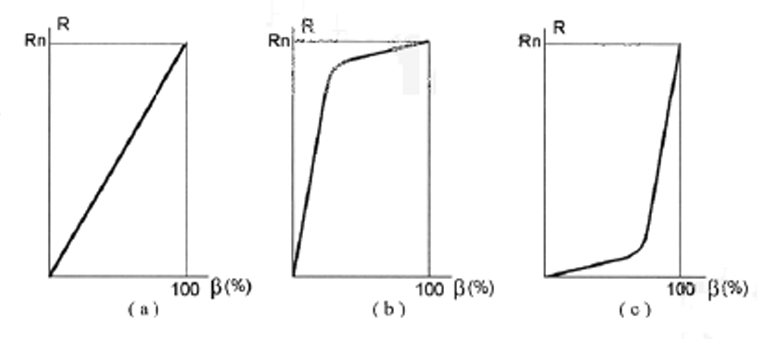
\includegraphics[width=0.75\linewidth]{Imagenes/Resistncias Potenciometros - Respuestas.png}
    \caption{Resistencias Ajustables. Potenciómetros.}
\end{figure}

\subsubsection{Tipos}

\begin{itemize}
    \item Bobinados de baja potencia.
    \item Bobinados de alta potencia.
    \item De capa de carbón.
    \item De capa metálica.
\end{itemize}

\subsubsection{Aplicaciones}

\begin{itemize}
    \item Resistencia variable ajustable
    \item Divisor de tensión
\end{itemize}

\section{Condensadores}

\subsection{Introducción}

Componente electrónico constituido por 2 placas metálicas, entre las que se dispone un dieléctrico (aislante). Es un componente reactivo (capaz de almacenar energía).

\begin{figure}[H]
    \centering
    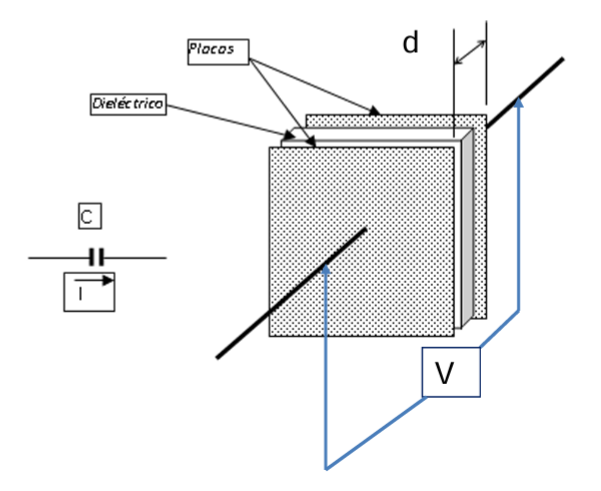
\includegraphics[width=0.5\linewidth]{Imagenes/Condensadores.png}
    \caption{Condensador - Estructura}
\end{figure}

La capacidad de un condensador se define como la carga eléctrica que puede ser almacenada por el mismo cuando es sometido a una diferencia de potencial. El material dieléctrico utilizado tiene una gran influencia en el valor de dicha capacidad.

\begin{equation}
    C = \frac{Q}{V}
\end{equation}

\begin{equation}
    I = C \frac{dU}{dt}
\end{equation}

\begin{equation}
    Zc = \frac{1}{j\omega C}
\end{equation}

\begin{equation}
    C = \xi_r \xi_0 \frac{A}{d}
\end{equation}

Donde:
\begin{itemize}
    \item $C$: Capacidad en faradios ($F$).
    \item $d$: Espesor del dieléctrico (en $m$).
    \item $A$: Superficie de las placas conductoras (en $m^2$).
    \item $\xi_r$: Permitividad relativa (depende del dieléctrico utilizado)
    \item $\xi_0$: Permitividad del vacío
\end{itemize}

\subsection{Parámetros Característicos}
\begin{itemize}
    \item Capacidad nominal (Cn).
    \item Tolerancia del valor capacitivo (+/- \% Valor nominal).
    \item Factor de calidad (D) (Factor de pérdidas). Cuando no hay pérdidas en el dieléctrico, la corriente está adelantada a la tensión $\pi / 2$ radianes. Las pérdidas originadas en el dieléctrico hacen que la corriente pase a estar adelantada a la tensión un ángulo menor ($90-\delta$)
    \begin{equation}
        Zc = \frac{1}{j\omega C}
    \end{equation}
    \begin{equation}
        D = tg \delta = \frac{R_S \vec{I}}{\vec{I}/\omega C} = R_S \omega C = R_s 2 \pi f C
    \end{equation}
    \item Tensión nominal en DC y AC. Tensión de trabajo a la que se puede someter el condensador.
    \item Rigidez dieléctrica. Voltaje máximo que puede soportar un dieléctrico sin perforarse ($V/m$). Las rupturas dieléctricas pueden ser de los siguientes tipos:
    \begin{itemize}
        \item Rupturas intrínsecas (avalancha interna de electrones)
        \item Térmicas
        \item De descargas
        \item Electroquímicas
    \end{itemize}
    \item Resistencia de aislamiento. Cuando un dieléctrico es sometido a una tensión continua $U$, presenta una corriente de fuga, $I_f$.
    \begin{equation}
        I_f = \frac{V}{R_i} [M\Omega \cdot \mu F]
    \end{equation}
    \item Coeficiente de temperatura. Variación de la capacidad nominal en función de la temperatura.
    \begin{equation}
        \alpha_C = \frac{1}{C} \frac{\Delta C}{\Delta T} \cdot 10^6 [ppm / ^\circ C]
    \end{equation}
    \item Categoría climática. El código de la categoría climática está formado por una serie de 3 números, separados por /, de la siguiente forma:
    \begin{equation}
        AA / BB / CC
    \end{equation}
    Los cuales indican:
    \begin{itemize}
        \item $AA$: Temperatura ambiente mínima de operación.
        \item $BB$: Temperatura máxima de operación.
        \item $CC$: Número de días sometidos a calor húmedo.
    \end{itemize}
\end{itemize}

\subsection{Condensadores de dieléctrico plástico}

\subsubsection{Características principales}

\begin{itemize}
    \item Tienen un volumen reducido.
    \item La resistencia de aislamiento, $tg \delta$ varía con la temperatura.
    \item Tienen un aislamiento elevado, lo que les permite conservar la carga eléctrica durante mucho tiempo.
    \item Tienen una débil absorción eléctrica, que permite cargas y descargas rápidas (Apropiados aplicaciones de alta frecuencia).
    \item Pueden venir en caja de plástico con terminales radiales o cilíndricos con terminales axiales.
\end{itemize}

\subsubsection{Proceso de Fabricación}
\begin{enumerate}
    \item Bobinado de las láminas de plástico y aluminio.
    \item Las láminas se hacen pasar por un peine electrostático para eliminar las cargas electrostáticas.
    \item El condensador se somete a una elevada temperatura, para contraer las láminas de plástico y expulsar la posibles burbujas de aire.
    \item Se sellan los extremos del arrollamiento para asegurar la estanqueidad del mismo.
\end{enumerate}

\subsection{Condensadores cerámicos}

Utilizan como material dieléctrico, un material cerámico. Diferenciamos:

\begin{itemize}
    \item CLASE 1: Se utilizan en aplicaciones en las que se requieran unas pérdidas muy bajas, y una elevada estabilidad, así como unas pérdidas bajas (osciladores y filtros).
    \begin{itemize}
        \item Elevada resistencia especifica.
        \item Factor de calidad D muy bueno.
        \item Comportamiento lineal con la temperatura
    \end{itemize}
    \item CLASE 2: Se utilizan en acoplo y desacoplo.
    \begin{itemize}
        \item Tienen pérdidas altas y comportamiento no lineal.
    \end{itemize}
\end{itemize}

\subsubsection{Características más importantes}
\begin{itemize}
    \item Resistividad: $\rho = 10$ a $10^{13}T\Omega \cdot cm$
    \item Factor de pérdidas: $tg \alpha = 10^{-3}$ a $10^{-4}$ a $1 MHz$.
    \item Rigidez dieléctrica: $35$ a $90 kV/cm$.
\end{itemize}

\subsubsection{Aplicaciones típicas}
\begin{itemize}
    \item Aplicaciones de AF.
    \item En desacoplo de alimentación (absorben rápidas variaciones de la VCC).
    \item Acoplo.
    \item Filtros
\end{itemize}

\subsubsection{Proceso de Fabricación}

\begin{enumerate}
    \item La materia prima se muele, se mezcla y se somete a un procesado a alta temperatura (1100 a 1300 ºC).
    \item Se solidifica el material con aglutinantes, obteniéndose unas láminas prensadas.
    \item Se imprime el electrodo en las láminas.
    \item Se hace el laminado con varios niveles mediante prensado y curado a 1400 ºC.
\end{enumerate}

\subsubsection{Estructura Interna}

Consiste en un bloque rectangular de material dieléctrico cerámico, formado por varios substratos de electrodos de metales preciosos. Permite obtener una elevada capacidad por unidad de volumen. Los electrodos internos están conectados a los dos terminales mediante una aleación plata/paladio en proporción de 65/35, o bien por recubrimiento formado por un estrato de plata, uno de níquel y posteriormente, un acabado de estaño (barrera de níquel).

\begin{figure}[H]
    \centering
    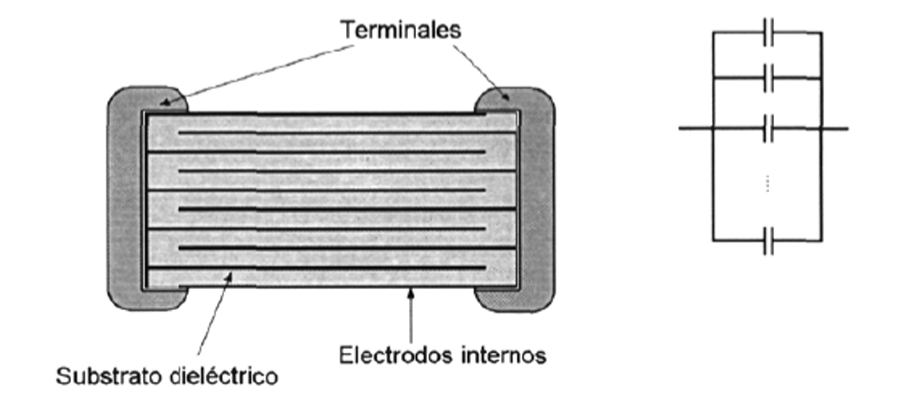
\includegraphics[width=0.5\linewidth]{Imagenes/Condensadores Ceramicos - Estructura Interna.png}
    \caption{Estructura Interna.}
\end{figure}

\subsection{Condensadores electrolíticos}

Utilizan como electrolito, una solución líquida que actúa como medio de transporte de la corriente entre los dos electrodos. Están polarizados y no admiten corrientes alternas. Están formados por:

\begin{itemize}
    \item Ánodo: Electrodo positivo de aluminio recubierto de alúmina (Al2 O3).
    \item Cátodo: Electrodo negativo formado por una lámina de aluminio de alta pureza.
    \item Electrolito: Tetraborato amónico impregnado en un papel especial.
    \item Dieléctrico: Alúmina (Al2 O3)
\end{itemize}

Para aumentar al máximo la capacidad, sin aumentar el volumen, se utilizan unas láminas con una superficie muy rugosa obtenida por procedimientos químicos. El papel soporte del electrolito es un papel de gran absorción, muy poroso y también corrugado.

\subsubsection{Parámetros Característicos}
\begin{itemize}
    \item Factor de pérdidas: El factor de pérdidas crece notablemente con la frecuencia, por lo que el uso de los condensadores electrolíticos debe limitarse a frecuencias menores a $10 kHz$.
    \item Corriente de fuga: Aumenta rápidamente a partir de tensiones superiores a $500 V$, y conforme aumenta la temperatura de servicio.
    \item Variación de la capacidad con la temperatura: La capacidad del condensador electrolítico se incrementa conforme aumenta la temperatura.
\end{itemize}

\subsubsection{Condensadores electrolíticos de Tántalo}

Utilizan un electrolito sólido. El dieléctrico generalmente utilizado es de óxido de tántalo (Ta2 O5). Se elaboran partiendo de un polvo de tántalo sintetizado (oxidado) que constituye material tipo P. Esta amalgama se recubre con bióxido de manganeso (MnO2), que se comporta como material N. El conjunto en definitiva constituye un semiconductor P-N.

\section{Dispositivos Inductivos}

Componente electrónico reactivo, capaz de almacenar cierta energía eléctrica. Presenta una inductancia (coeficiente de autoinducción) $L$ (Henrios). Su comportamiento se basa en la teoría electromagnética. La tensión en sus bornas es adelantada $\pi / 2$ respecto de la intensidad.

\begin{equation}
    V = -L \frac{di}{dt}
\end{equation}

\begin{equation}
    V = -N \frac{d\phi}{dt}
\end{equation}

El modelo equivalente incorpora una componente resistiva en serie con la bobina causante de ciertas pérdidas.

\begin{equation}
Q = tg \phi = \frac{\omega L I}{RI} = \frac{\omega L}{R}
\end{equation}

\subsection{Parámetros Característicos}

\begin{itemize}
    \item Densidad de flujo magnético ($B$) [$Wb/m^2$]. Flujo magnético $\Phi$ contenido en una sección $A$ del núcleo.
    \begin{equation}
        B = \frac{\Phi}{A} = \frac{\mu_0 I}{2\pi r}
    \end{equation}
    \item Fuerza de magnetización ($H$)[$A/m$]. Energía eléctrica necesaria para producir una determinada densidad de flujo magnético ($B$).
    \begin{equation}
        H = \frac{NI}{P}
    \end{equation}
    \item Permeabilidad magnética ($\mu$)[$Wb$][$H/m$]. Facilidad para conducir el flujo magnético. 
    \begin{equation}
        \mu = B/H
    \end{equation}
    \item Permeabilidad del vacío ($\mu_0$): $\mu_0 = 4 \cdot \pi \cdot 10^{-7} H/m$.
    \item Permeabilidad relativa ($\mu_r$): $\mu_r = \frac{\mu}{\mu_0}$
\end{itemize}



\subsection{Ferritas}
\subsubsection{Composición}
Se elaboran con aleaciones de distintos metales (Mn, Zn, Ni, Co, Cu, Fe, Mg). Los más usuales MzZn y NiZn, mezclados con materiales cerámicos. Tienen un aspecto cerámico de color oscuro. Duras, frágiles y químicamente inertes. Presentan una alta resistividad a altas frecuencias. Tienen una alta permeabilidad ($\mu$).

\subsubsection{Proceso de Fabricación}

\begin{enumerate}
    \item Obtención de la materia prima (aleaciones), en distintas proporciones, en forma de polvo.
    \item Presinterización a unos 1000ºC para unificación del material.
    \item Molido y granulado a un tamaño determinado de las partículas, incluyendo agua y apelmazante.
    \item Conformado a la geometría definitiva por moldeado, mediante compresión.
    \item Sinterización final para la solidificación del material (eliminación de productos residuales) y obtener las características magnéticas requeridas.
    \item Magnetización final mediante campo magnético externo.
    \item Acabado (mecanizado) final de la pieza.
\end{enumerate}

\subsubsection{Aplicaciones}

\begin{itemize}
    \item Filtro tipo pasabanda
    \item Supresión de interferencias: Permite el bloqueo de señales de ruedo indeseables.
    \item Retardo de pulso: Permite retrasar el pulso ascendente de una señal un intervalo de tiempo determinado por el componente inductivo.
    \item Almacenamiento de energía: Permite almacenar energía y entregarla posteriormente a la carga, durante el tiempo en off de una fuente de alimentación conmutada.
\end{itemize}

\section{Cristales de Cuarzo}